\documentclass[11pt, a4paper]{article}

\usepackage[T1]{fontenc}
\usepackage[utf8]{inputenc}

\usepackage[ngerman]{babel} %Silbentrennung, ‚Ueberschriften wie Inhaltsverzeichnis, Bilder, Tabellen werden deutsch angeschrieben
\usepackage{csquotes}
\usepackage{graphicx} %um grafiken einbinden zu können
\usepackage{float} %erlaubt zB. einen Rahmen um eine Float-Umgebung zu zeichnen
\usepackage{endnotes} %Für Endnoten
\usepackage{pifont} %Erlaubt die Verwendung von speziellen Symbolen via \ding{nummer}
\usepackage{hyperref} %macht aus \ref klickbare links, erlaubt den Gebraucht von \nameref{}
\usepackage{booktabs, threeparttable} %booktabs erlaubt \toprule, \midrule, \bottomrule. threeparttable ist u.a. dazu da, dass man die caption so breit wie die tabelle haben kann.


% Mit den folgenden 3 Parametern kann man das Verhalten von LaTeX in Bezug auf Gleitumgebungen/Text steuern. Normalerweise ist es nicht moeglich, eine einzelne Seite nur mit floats zu fuellen. Passt man aber folgende Parameter an, erlaubt man LaTeX mehrere Floats auf einer Seite zu platzieren, auch wenn nur sehr wenig dieser Seite mit Text gefuellt ist

\renewcommand{\textfraction}{0.001}
\renewcommand{\topfraction}{0.999}   
\renewcommand{\bottomfraction}{0.999}

% Paket um mit Tikz zeichnen zu koennen
\usepackage{tikz}

% Mathpackages
\usepackage{amsmath} 
\usepackage{amsfonts}
\usepackage{amssymb}
\usepackage[top=2.5cm, left=2cm, right=2.5cm, bottom=2cm]{geometry}
\usepackage{a4}

% Indexverzeichnis
\usepackage{makeidx}
\makeindex

% Bibliographie Packages
\usepackage[style=authoryear, backend=biber, maxnames=5]{biblatex}
\addbibresource{bibliography.bib}


\pagestyle{headings} %standard headings. Andere optionen: plain, empty

\newcommand{\ltx}{\LaTeX}
%\linespread{1.2}\selectfont % Global Zeilenabstände ändern

\setlength{\belowcaptionskip}{2ex}
\setlength{\abovecaptionskip}{1ex}

% Neudefinition von Marginalien
% Mehr Info hier: http://tex.stackexchange.com/questions/48571/redefine-marginpar-with-renewcommand
\let\oldmarginpar\marginpar
\renewcommand{\marginpar}[1]{\oldmarginpar{\textit{#1}}}




% Titelseite
\title{\ltx{} leicht gemacht}
\author{Hans Muster\\ Universität Hier\thanks{hans.musterman@uni-hier.edu} \and Peter Lustig\\Universität Dort\thanks{peter.lustig@uni-dort.edu}}

% Dokumentbeginn
\begin{document}

\maketitle
\tableofcontents
\newpage

\section{Einfacher als sein Ruf}

Für ein einfaches \ltx-Dokument braucht es nur eine Hand voll Befehle. Nicht einmal um die Formatierung müssen Sie sich kümmern, sondern können sich voll und ganz dem Text widmen.

Den grössten Teil des Fliesstextes können sie wie gewohnt eingeben, nur wenige Sonderzeichen\index{Sonderzeichen} benötigen spezielle Befehle. Dank dem Zusatzpaket ngerman können sie Umlaute als \verb+"+a (ä), \verb+"+o (ö), etc. eingeben. Es gibt auch Möglichkeiten, die Umlaute einzutippen, wie Sie es sich gewohnt sind (Zusatzpaket fontenc/inputenc), jedoch sind diese \ltx-Dokumente dann nicht mehr plattformübergreifend funkionsfähig.

\section{Einfache Textformatierung}

Einen neuen Absatz erzeugen Sie, indem Sie im Code (mindestens) eine Leerzeile einfügen. Dabei spielt es keine Rolle, ob es sich um eine oder zehn Leerzeilen handelt. Sie können so also keine vertikalen Abstände erzeugen; dazu werden spezielle Befehle benötigt.

\subsection{Silbentrennung und Trennstriche}

Um die Silbentrennung brauchen Sie sich grösstenteils gar nicht zu kümmern, das erledigt \ltx{} für Sie. Natürlich gibt es Ausnahmen, wo sie \ltx{} mit den korrekten Trennstellen auf die Sprünge helfen müssen.

Trennstriche geben Sie ein wie gewohnt, wohingegen Gedanken- bzw. Streckenstriche (sogennante Halbgeviertsstriche) -- sollten Sie solche benötigen -- mit \verb+--+ erzeugt werden. Auch die doppelt so langen Geviertsstriche (---) können Sie erzeugen (\verb+---+). Während diese im englischsprachigen Amerika als Gedankenstriche verwendet werden, finden sie sich in deutschsprachigen Dokumenten nur in Tabellen bei Währungsbeträgen wieder.

\subsection{Anführungen}
Anführungszeichen\index{Anführungszeichen!Gänsefüsschen} werden in \ltx{} traditionellerweise mit \`{}\`{} \verb+''+ (`` '') erzeugt, was jedoch die in Amerika üblichen Anführungszeichen generiert. Gebräuchlicher bei uns sind die deutsche "\`{} "\verb+'+ ("` "') oder die französische Anführung \verb+"< ">+ ("< ">).

\begingroup
\setlength{\parindent}{0pt}
\setlength{\parskip}{1.5ex plus 0.5ex minus 0.2ex}
\section{Textformatierung\label{sec:eftf}}

\subsection{Zeichen}

\subsubsection{Deutsche Spezifika}
Die deutschen Umlaute ä, ö, ü, Ä, Ö und Ü sind in den deutschsprachigen Texten natürlich überall zu finden. Auch die "`Gänsefü\ss chen"' sollten Sie in dieser korrekten Weise setzen.

\subsubsection{Andere Sonderzeichen}
Häufiger benötigen Sie einige Akzentzeichen, z.B. Acute-Akzent é und der Grave-Akzent à. Bei rechtlichen Fragestellungen werden Sie auch das §-Zeichen benötigen. Fortsetzungspunkte (\dots) und Gedankenstriche (--) werden mit speziellen \ltx-Befehlen gesetzt.

\subsection{Absätze}
Dieser Text enthält sowohl Absätze auch einfach Zeilenumbrüche. Für den Abschnitt \ref{sec:eftf} (beginnend auf Seite \pageref{sec:eftf}) wurde vereinbart, dass für die erste Zeile eines Absatzes keinen Einzug verwendet wird.

\begingroup
\raggedright %für linksbündig
Der Abstand zwischen den Absätzen soll 1.5ex betragen, der um maximal 0.5ex aufgeweitet und um höchstens 0.2ex gestaucht werden kann. Dieser und der folgende Absatz sollen linksbündig ausgerichtet werden.

\vspace{1cm}
\subsection{Sonstiges} 
Hier wurde $1$\,cm \fbox{zusätzlicher} Platz vor dem Absatz eingesetzt. 
\endgroup
\endgroup

\section{Visuelle Formatierung}
Beim grössten Teil der Formatierbefehle im Abschnitt~\ref{sec:eftf} \nameref{sec:eftf} handelt es sich um \textit{visuelle Formatierung}, d.h. die Formatierbefehle\index{Formatierbefehle!Beispiel} beschreiben, wie der Text \textit{aussehen} soll. In der Praxis werden sie Ihre Texte \textsc{\textbf{nie}} auf diese Weise formatieren (ausser in wenigen wohlbegründeten Ausnahmen).
Stattdessen verwenden Sie Befehle zur \textit{logischen Formatierung} (häufig auch generische Formatierung genannt), die beschreiben, welchen Stellenwert ein bestimmter Textteil in Bezug auf die Dokumentstruktur oder den Inhalt hat\index{Sonderzeichen}.

\section{Schriften mit \ltx}

Der Schriftstil wird in \ltx{} durch 3 Merkmale definiert:

\begin{enumerate}
\item Schriftfamilie
\begin{itemize}
\item Serifenschriften (roman): proportionale Schriften mit kleinen Hilfslinien an jedem Buchstaben auf H\"ohe der Schriftlinie (Serifen);
\item \textsf{serifenlose Schriften: proportionale Schriften ohne Hilfslinien auf der Schriftlinie};
\item \texttt{Schreibmaschinenschriften: Alle Zeichen haben die gleiche Breite (diktengleich)};
\end{itemize}
\item Schriftst\"arke:
\begin{itemize}
\item normale Schriftstärke
\item \textbf{fette Schriften\index{fett|textbf}}
\end{itemize}
\item Schriftform:
\begin{itemize}
\item aufrechte Schriften
\item \textsl{geneigte Schriften}
\item \textit{kurisve Schriften}
\item \textsc{Schriften in Kapitälchen}
\end{itemize}
\end{enumerate}

Auch wenn in \ltx{} viele Befehle existieren, mit welchen sich Schriftaren, Schriftgrössen und Schriftformen manipulieren lassen, sollte man sich eine allgemeingültige Aussage immer vor Augen halten:
\begin{quote}
Typographisches Design ist ein Handwerk, das erlernt werden muss. Ungeübte Autoren machen dabei oft gravierende Fehler. Fälschlicherweise glauben viele Laien, dass Textdesign vor allem eine Frage der Ästhetik sei: Sobald das Schriftstück "`schön aussehe"', sei das Ziel erreicht. Da Schriftstücke jedoch gelesen werden und nicht als Kunstwerke in einem Museum aufgehängt werden sollen, sind die leichtere Lesbarkeit und bessere Verständlichkeit jedoch viel wichtiger als das "`schöne Aussehen"'.
\end{quote}

\noindent Wir geben Ihnen hier noch einige Tipps, an welche Sie sich beim Erstellen Ihrer Dokumente halten sollten:
\begin{itemize}
\item[\ding{43}] Umfangreiche Texte sollten Sie in einer Serifenschrift setzen.
\item[\ding{43}] Hervorhebungen in einem Text können Sie durch \textsl{geneigte Schriften} oder durch \textit{kursive Schriften} vornehmen. \textit{Kursive Schriften} sind durch ihre andere Gestaltung meist etwas auffälliger als die \textsl{geneigten Schriften}. \textbf{Fette Schriften} betonen dagegen sehr stark.
\item[\ding{43}]  \textsf{Serifenlose Schriften sind hingegen gut geeignet für Überschriften und plakative Texte}
\item[\ding{43}] Weniger ist oft mehr: Vermeiden Sie die den häufigsten Fehler im Umgang mit \ltx! Überlassen Sie die Formatierung Ihrer Texte \ltx{} und verwenden Sie Ihre Arbeitszeit zum Verfassen Ihrer Texte.
\end{itemize}


\begin{table}[t]
\caption{Mustertabelle zur Aufgabe 8  \label{tab:Schriftgroessen}}
\centering
\begin{tabular}{lccc}
\toprule
\textbf{\ltx-Befehl} & \multicolumn{3}{c}{\textbf{Basisschriftgrösse}}\\
\cline{2-4} & \textbf{10pt} & \textbf{11pt} & \textbf{12pt}\\
\midrule
\midrule
\verb+\tiny+			& 5pt & 6pt 	& 6pt\\
\verb+\scriptsize+		& 7pt & 8pt		& 8pt\\
\verb+\footnotesize+	& 8pt & 9pt		& 10pt\\
\verb+\small+			& 9pt & 10pt	& 11pt\\
\midrule
\midrule
\verb+\normalsize+		& 10pt	& 11pt	& 12pt\\
\midrule
\midrule
\verb+\large+			& 12pt	& 12pt	& 14pt\\
\verb+\Large+			& 14pt	& 14pt	& 17pt\\
\verb+\LARGE+			& 17pt	& 17pt	& 20pt\\
\verb+\huge+			& 20pt	& 20pt	& 25pt\\
\verb+\Huge+			& 25pt	& 25pt	& 25pt\\
\bottomrule
\end{tabular}
\end{table}%

\section{Ein Tabellenbeispiel}
Tabelle \ref{tab:Schriftgroessen} stellt die real benutzten Schriftgrössen für die \ltx-Schriftgrössenbefehle in Abhängigkeit von der Basisschriftgrösse dar.\par
Die kleinste darstellbare Schrift ist 5pt, die grösste 25pt hoch. Die Schriften werden in der Regel in diskreten, gut miteinander harmonierenden Grössen benutzt.

\section{Bilder in \ltx}
\ltx{} erlaubt die Erstellung von Grafiken direkt mit \ltx-Befehlen als auch die Einbettung von extern erzeugten Grafik-Dateien. Zu beiden Varianten werden nachfolgend Beispiele gezeigt.




\subsection{Strichgrafiken mit \ltx-Befehlen}

\ltx{} erlaubt die Erstellung von Grafiken direkt mit \ltx-Befehlen. Ein Beispiel dazu zeigt Abbildung \ref{fig:tikz}. Tikz ist ein zus"atzliches Paket, das in der Pr"aambel geladen wird.
Mit Tikz sind die Moeglichkeiten fast zahllos, man muss ledliglich eine Idee haben, die man umsetzen will. F"ur mehr Informationen zu Tikz kann man diese minimale Einf"uhrung in Tikz durchlesen:
\url{http://cremeronline.com/LaTeX/minimaltikz.pdf}
%
\begin{figure}[t]
\centering
\begin{tikzpicture}[scale=0.6]
% Koordinatensystem
\draw [->] (-5,0) -- (5,0);
\draw [->] (0,-5) -- (0,5);

% Beschriftung vom Koordinatensystem
\node [below] at (5,0) {$x$};
\node [left] at (0,5) {$y$};

% Wiederholte vertikale Linien im 1. Quardrant
\foreach \x in {0.25, 0.5, 0.75,...,3} {
\draw (\x, 0) -- (\x, 3);
}

% Das Viereck - cycle schliesst den letzten Punkt mit dem ersten Punkt
\draw (-3,-3) -- (-3,3) -- (3,3) -- (3,-3) -- cycle;

% Einfache diagonale Linie
\draw (-4,-4) -- (4,4);

% Aufteilung der Koordinatenachse, fuer x und y - einfach jeweils die Argumente vertauscht
\foreach \t in {-4,-3,...,4}{
\draw (\t, -0.2) -- (\t, 0.2);
\draw (-0.2,\t) -- (0.2,\t);
}
\end{tikzpicture}
\caption{Eine Tikz-Grafik\label{fig:tikz}}
\end{figure}


\subsection{Etwas Geschichte -- Einbettung von Grafiken}
Am Anfang stand ein Buchprojekt. Der Informatik-Professor Donald Knuth setzte den ersten Band seines Werkes "<The Art of Computer Progrmaming"> 1969 mit Monotype, eine Technologie aus dem 19. Jahrhundert. Als 1976 der zweite Band erscheinen sollte, war die Monotype-Technologie mehrheitlich durch den fotografischen Textsatz ersetzt worden. Als Knuth die ersten Proof-Bögen erhielt, fand er diese schrecklich. So begann er 1977 damit, ein eigenes Textsatzsystem zu schreiben -- \TeX war geboren.

\begin{figure}[htb]
\centering
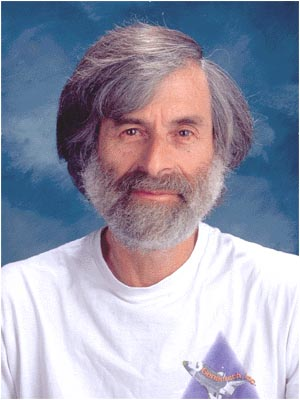
\includegraphics[width=0.2\textwidth]{Leslie_Lamportd}
\caption{Leslie Lamport\label{fig:LL}}
\end{figure}

\TeX{} bietet sehr viele Möglichkeiten zur Textformatierung, ist jedoch schwierig und umständlich in der Anwendung. Der Informatiker Leslie Lamport (siehe Abbildung \ref{fig:LL}) war jedoch der Meinung, ein Author solle sich vor allem auf seinen Text konzentrieren und sich nicht mit Formatierungen herumschlagen müssen. So begann er 1984 damit, ein Makropaket zu \TeX{} zu entwickeln, das dem Benutzer viele Formatierungsentscheidungen und sonstige Aufgaben abnimmt -- \ltx{}.

\section{Grundelemente des Formelsatzes}

Wissenschaftliche Arbeiten mit vielen Formeln stellen hohe Ansprüche an das Textsystem, denn mathematische Ausdrücke und Formeln werden anders behandelt als der normale Fliesstext. Ein Schwerpunkt bei der Entwicklung von \TeX{} und \ltx{} lag auf einem hochwertigen, den wissenschaftlichen und mathematischen Konventionen entsprechenden Formelsatz. Demzufolge bietet \ltx{} standardmässig viele Möglichkeiten, mathematische Formeln zu setzen.

\begingroup
\floatstyle{boxed}
\restylefloat{figure}
\begin{figure}[p!] %p erzielt, dass die figure auf einer Seite speziell für floats platziert wird
Gegeben sei die Funktionenschar
\begin{displaymath}
f_a(x) = \frac{x+a}{x^2}~\mbox{mit } a \in \mathbb{R}
\end{displaymath}
\begin{enumerate}
\item Untersuchen Sie die Funktionenschar \( f_a\) auf ihre maximale Definitionsmenge \(\mathbb{D}\). Bestimmen Sie alle Asymptoten der Graphen sowie das Verhalten der Graphen an den Grenzen des Definitionsbereichs.
\item Weisen Sie nach, dass zwei verschiedene Graphen der Schwar keinen gemeinsamen Punkt besitzen, aber sich für \(x\to\infty\) beliebig nahe annähern.
\item Zeichnen Sie den Graphen \(G_{f_1}\) im Intervall \(I = \left[-4;4\right]\) in ein geeignetes Koordinatensystem.
\item Zeigen Sie, dass
\begin{displaymath}
F(x) = x +(x+1)\cdot\ln(x+1) - 2x\cdot\mbox{ln}(x)
\end{displaymath}
eine Stammfunktion zu \(\displaystyle g(x) = \ln\left(\frac{x+1}{x^2}\right)\) ist.
\item Bestimmen Sie eine integralfreie Darstellung für die Integralfunktion

\[ F_x(x) = \int\limits_2^x\ln(f_1(t))\mathrm{d}t \]
\end{enumerate}
\caption{Ein einfaches Aufgabenblatt für Mathematiker}
\label{fig:formeln}
\end{figure}
\endgroup

Es mag zunächst verwundern, was \ltx{} alles unter die Rubrik Formelsatz stellt. Hierzu gehören u.a.
\begin{itemize}
\item Zahlen, Variablen, Operatoren
\item mathematische Symbole
\item Namen von Funtkionen
\item griechische Buchstaben
\item das Hoch- und Tiefstellen von Zeichen und Texten
\item komplette mathematische Formeln
\item diverse Sonderzeichen
\end{itemize}

Dabei werden Zahlen und Operatoren in einer aufrechten Schrift, Variablennamen meist in einer kursiven Schrift ohne Kerning gesetzt.

Ein wichtiges Zusatzpaket für den Formelsatz ist das von der American Mathematical Society (\AmS) entwickelte Paket \textit{amsmath}, das neben weiteren Operatoren und Symbolen auch zusätzliche Strukturelemente und Gestaltungsmöglichkeiten beinhaltet. Es empfielt sich, dieses Zusatzpaket standardmässig mit einzubinden. Dazu muss es mittles \verb+\usepackage{amsmath}+ in der Präambel des \ltx-Dokuments geladen werden.

Abbildung \ref{fig:formeln} zeigt eine Auswahl von Formelbefehlen. Ausserdem wird hier deutlich, dass in einer figure-Umgebung nicht zwingend ein Bild (im technischen Sinne) enthalten sein muss.

\clearpage %beginnt eine neue Seite und platziert alle noch nicht gesetzten Floats

\section{Fussnoten und Marginalien}

Nachfolgend finden Sie ein Zitat aus dem Lehrbuch, ergänzt durch einige Anmerkungen der Kursautoren -- themabezogen als Fussnoten\marginpar{Fussnoten}:

\begin{quote}
Längere, zusätzliche Erklärungen werden meist nicht im Fliesstext eingefügt, da auf diese Weise schnell der Sinnzusammenhang verloren gehen kann. Stattdessen wird durch eine Markierung -- meist eine kleine hochgestellte Zahl\footnote{Üblicherweise in aufsteigender Reihenfolge.} -- auf sie verwiesen\footnote{Beachten Sie aber, dass auch eine Fussnote den Lesefluss beträchtlich stören kann. Wägen Sie immer ab, ob Sie die Anmerkung wirklich brauchen und ob diese im Fliesstext nicht besser aufgehoben wäre.}. Im Seitenfuss wird diese Markierung wiederholt und der erklärende Text in einer kleinen Schriftgrösse\footnote{Eben in der Grösse \textbackslash\texttt{footnotesize}.} ausgegeben. Zur deutlichen Trennung zwischen dem Fliesstext und den Fussnoten wird zwischen diesen Seitenbereichen eine kurze horizontale Linie mit entsprechendem Leerraum gesetzt\footnote{Es gibt auch Publikationen, wo diese Linie über die ganze Seitenbreite ausgezogen wird.}.

Im Fliesstext können Sie mit \ltx{} relativ einfach Fussnoten anbringen. Die Nummerierung wird dabei automatisch von \ltx{} verwaltet, so dass es auch im Nachhinein möglich ist, Fussnoten neu einzufügen oder zu löschen\footnote{Weiter verwaltet \ltx{} auch die Seite, wo der Fussnotentext erscheint. Dieser sollte immer auf der selben Seite stehen, wie die Fussnotenmarkierung. \ltx{} gelingt dies fast immer (ausser in einigen verzwickten Fällen), wohingegen Microsoft Word hier überdurchschnittlich oft scheitert.}. Die Nummerierung wird mit jedem Kapitel (Dokumentklassen \textit{report} und \textit{book}) wieder zurückgesetzt, so dass die Nummerierung der Fussnoten wieder bei Eins beginnt. Fussnoten können auch innerhalb der \textit{minipage}-Umgebung verwendet werden.

Auf Grund der \ltx-internen Bearbeitung der Fussnoten gibt es einige Dokumentteile, in denen dieser Automatismus nicht korrekt funktioniert: z.B. in Tabellen, Gleitumgebungen, mathematischen Ausdrücken, \ltx-Boxen. In diesen Fällen bedarf es eines Umweges, um dort Fussnoten anzubringen.
\end{quote}

Auch bei Endnoten\marginpar{Endnoten} handelt es sich um erklärende Texte, die im Gegensatz zu Fussnoten aber gesammelt am Ende des Kapitels oder des Dokuments ausgegeben ewrden. Gerade bei längeren Anmerkungen oder vielen Anmerkungen pro Seite kann sich der Einsatz von Endnoten lohnen. \ltx{} benötigt für Endnoten \parencite{lkgt} -- im Gegensatz zu Fussnoten -- ein Zusatzpaket: \texttt{endnotes}. Da Endnoten tendentiell eher seltener als Fussnoten verwendet werden, werden wir in dieser Übung auf Endnoten verzichten.

Marginalien\marginpar{Marginalien} sind in einem gewissen Sinne ebenfalls Anmerkungen. Allerdings handelt es sich dabei nicht um längere, erklärende Texte, sondern eher um Hinweise, um bestimmte Stellen im Text zu kennzeichnen.

\section{Literaturhinweise mit Bib\LaTeX}
Bibliographie-Erstellung mit dem Zusatzprogramm Bib\LaTeX{} bedeutet, dass Sie Ihre Literatur in separaten Textdateien erfassen, welche als Bibliographie- dateien bezeichnet werden. Sie können zur Verbesserung der Übersichtlichkeit separate Bibliographiedateien für verschiedene Themengebiete anlegen.

Die einzelnen Referenzen schreiben Sie in die Dateien im Bib-Format, das eines der meistbenutzten Formate für Bibliographiesammlungen im Textformat ist und auch von anderen Programmen weiterverarbeitet werden kann. Bib-Dateien lassen sich z.B. bequem mit dem Programm "<JabRef"> bearbeiten, welches als Java-Applikation plattformübergreifend verfügbar ist.
Das Programm Bib\LaTeX{} erledigt dann folgende Aufgaben für Sie:
\begin{itemize}
\item Erstellung einer Liste aller im Text zitierter Dokumente
\item Unterstützung für die Hinzunahme weiterer, nicht zitierter Dokumente
\item Auswahl aus verschiedenen Layoutstilen, die Sie auch ändern oder komplett selber schreiben können (was allerdings absolut nicht trivial ist!)
\item Automatische Formatierung der Referenzen gemäss dem gewählten Layoutstil
\item Sortierung der Literaturliste
\item Unterstützung von verschiedenen Referenzformen im Text
\item Syntaxprüfung der Bibliographiedatei
\item Prüfung der Eindeutigkeit von Schlüsseln
\end{itemize}
Mit der Benutzung von Bib\LaTeX{} gewinnen Sie aber mehr als das: Wer Bibliographiedateien im Bib-Format in grossem Ausmass benutzt wird es schnell als gutes Mittel zur Bibliographieverwaltung schätzen lernen. Als textbasiertes System, für das diverse graphische Oberflächen existieren (z.B: "<JabRef">), ist es auch gut zum Nachschlagen oder Austausch mit Kollegen. Da Sie beliebig weitere Felder hinzufügen können, ist es auch geeignet, um z.B. Quellenangaben oder Bibliotheksstandorte zu notieren, Schlüsselwörter zu vergeben, usw.


\section{Indices}
Lassen Sie uns zuerst Leslie Lamport, den Autoren von \ltx{} zum Thema zum Wort kommen:
\begin{quote}
Der Index soll dem Leser helfen, bestimmte Informationen im Dokument zu finden, und zwar so einfach wie möglich. Viele Verfasser indizieren Wörter, indem sie alle Seiten, auf denen ein bestimmter Begriff erscheint, auflisten. Ein guter Autor erstellt einen Index nach Konzepten -- Ideen, Fakten, Personen usw.

Zur Erstellung eines Index müssen Sie sich zunächst überlegen, welche Konzepte Sie dort aufführen wollen. Danach müssen Sie herausfinden, nach welchen Schlagworten sich der Leser vermutlich orientiert, um ein Konzept zu finden. Sie müssen sich überlegen, welche Leserschaft das Buch haben wird, und wie die Leser das Konzept auffassen. Beschränken Sie sich nicht auf die Auflistung der Wörter, die Sie selbst zur Beschreibung des Konzeptes verwendet haben.

Sie sind vielleicht versucht, das Stichwortverzeichnis bereits beim Schreiben des Dokumentes anzulegen. Widerstehen Sie dieser Versuchung. Es ist nahezu unmöglich, auf diese Weise einen guten Index zu erstellen. Fügen Sie beim Schreiben \verb+\index+-Befehle ein, damit Sie sich später daran erinnern, für welche Begriffe Sie Indexeinträge erstellen wollten, aber bereiten Sie sich darauf vor, diese Befehle noch einmal zu überarbeiten, wenn Sie den Index erstellen.
\end{quote}
Nehmen Sie sich diese Aussagen unbedingt zu Herzen\cite{dlb}, denn wie Sie auch an einem kurzen Text schon sehen können, nützt ein Index, wo jedes Vorkommen eines bestimmten Stichwortes aufgelistet wird, nicht sonderlich viel. Trotzdem wollen wir in diesem Beispieltext gleich davon abweichen, denn hier soll es um die Anwendung der Index-Befehle und nicht um das Endresultat gehen.

\begin{table}[h!]
\centering
\caption{Übersicht der Indexierbefehle\label{tab:Indexbefehle}}
\begin{tabular}{lll}
\toprule
Example &	Index Entry	 & Comment\\
\midrule
\verb+\index{hello}+ &	hello, 1	& Plain entry \\
\verb+\index{hello!Peter}+	&  Peter, 3	 &Subentry under 'hello'\\
\verb+\index{Sam@\textsl{Sam}}+&	\textsl{Sam}, 2	&Formatted entry\\
\verb+\index{Lin@\textbf{Lin}}	+&	\textbf{Lin}, 7	&Same as above\\
\verb+\index{Jenny|textbf}+&	Jenny, \textbf{3}	&Formatted page number\\
\verb+\index{Joe|textit}+&	Joe, \textit{5}	&Same as above\\
\verb+\index{ecole@\'ecole}+&	école, 4&	Handling of accents\\
\verb+\index{Peter|see{hello}}+&	Peter, \textit{see} hello	&Cross-references\\
\verb+\index{Jen|seealso{Jenny}}+ &	Jen, \textit{see also} Jenny	&Same as above\\
\bottomrule

\end{tabular}

\end{table}%

\newpage

\printbibliography
\printindex
\end{document}
